If crossing conditions are not fulfilled we have a couple of options:
\begin{itemize}
	\item If initial curve is characteristic curve, we have infinite number of solutions.
	\item If initial curve is not characteristic curve, but their projection on $xy$-plane is same, we have no solution, since each solution includes characteristic curve.
\end{itemize}

In other cases, if for example initial curve is tangent to characteristic curve and their projection on $xy$-plane are different, there are different possibilities.

\paragraph{Example}
$$yu_x - xu_y = 0$$
with initial curve $(s,0,h(s))$ and $0<\alpha\leq s\leq \beta$
\subparagraph{Solution}
$$\begin{cases}
\dot{x} = y\\
\dot{y} = -x\\
\dot{z} = 0
\end{cases} \Rightarrow \begin{cases}
\ddot{x} = -x\\
\ddot{y} = -y\\
\dot{z} = 0
\end{cases} \Rightarrow \begin{cases}
x = A(s)\sin(t)+B(s)\cos(t)\\
y = A(s)\cos(t)-B(s)\sin(t)\\
z = c
\end{cases}$$
Now from initial curve
$$A(s)= s \quad B(s) = 0$$
$$ \begin{cases}
x = s\cos(t)\\
y = -s\sin(t)\\
z = h(s)
\end{cases}$$
Now we want to find $s$, $t$ as a function of $x$,$y$:
$$x^2+y^2 = s^2 \Rightarrow s = \sqrt{x^2+y^2}$$
$$u(x,y)  = h\left(\sqrt{x^2+y^2}\right)$$
Note that characteristic curves are rings.

\paragraph{Example}
$$yu_x - xu_y = u$$
with initial curve $(s,0,h(s))$ and $0<\alpha\leq s\leq \beta$
\subparagraph{Solution}
$$\begin{cases}
\dot{x} = y\\
\dot{y} = -x\\
\dot{z} = u
\end{cases} \Rightarrow \begin{cases}
\ddot{x} = -x\\
\ddot{y} = -y\\
z = C(s)e^t
\end{cases} \Rightarrow \begin{cases}
x = A(s)\sin(t)+B(s)\cos(t)\\
y = A(s)\cos(t)-B(s)\sin(t)\\
z = C(s)e^t
\end{cases}$$
Now from initial curve
$$A(s)= s \quad B(s) = 0$$
$$ \begin{cases}
x = s\cos(t)\\
y = -s\sin(t)\\
z = h(s)e^t
\end{cases}$$
Now we want to find $s$, $t$ as a function of $x$,$y$:
$$x^2+y^2 = s^2 \Rightarrow s = \sqrt{x^2+y^2}$$
And
$$\tan t  = -\frac{y}{x} \Rightarrow t = \arctan \left(-\frac{y}{x}\right)$$
$$u(x,y)  = h\left(\sqrt{x^2+y^2}\right)e^{ \arctan \left(-\frac{y}{x}\right)}$$


\subsection{Burgers' equation}
$$u_y + uu_x = 0$$
(which is partial case of equation of form $$\pdv{u}{y} + \pdv{ y} F(u) = 0$$ for $F=\frac{1}{2}u^2$)

Note that $$\frac{u_y}{u_x} = -u \Rightarrow \dv{x}{y} = - u \Rightarrow u = -\dv{x}{y}$$
Here $y$ denotes time.

To solve it, we take integral:
$$\int_a^b \left[ \pdv{ u(x,y)}{y} + \pdv {x} F(u(x,y))\right] \dd{x} = 0$$
$$\pdv{y} \underbrace{\int_a^b u \dd{x}}_{Q(y)}  + F\Big(u(b,y)\Big) - F\Big(u(a,y)\Big) = 0$$
$$\dv{Q}{y} = F\Big(u(a,y)\Big) - F\Big(u(b,y)\Big)$$

Now as for any quasilinear PDE:
$$\begin{cases}
\dot{x}= z\\\dot{y} = 1\\\dot{z}= 0
\end{cases} \Rightarrow \begin{cases}
x= c_2 t + c_3\\y = t + c_1\\\dot{z}= c_2
\end{cases} $$
For initial conditions $\Big(s,0,h(s)\Big)$:
$$ \begin{cases}
x= h(s) t + s\\y = t \\z= h(s)
\end{cases} $$
Now 
$$s=x-yu \Rightarrow u = h(x-yu)$$
Checking transversality condition:
$$\dv{\bar{x}}{s} \cdot 1 - \dv{\bar{y}}{s} \cdot h(s) = 1 \neq 0$$  


Since
$$\pdv{u}{x} = h'(x-yu) \cdot \left(1 - y\pdv{u}{x} \right)$$
$$\pdv{u}{x} = \frac{h'(x-yu)}{1+h'(x-yu) \cdot y} $$
even if we start from $\mathcal{C}^\infty$ function we can get $1+h'(x-yu) \cdot y = 0$ and thus undefined derivative.

Geometrically, the slope of projections of characteristic curves is equal to $h(s)$ thus they can cross in some point.

\paragraph{Weak solutions}
We define a weak solution of equation, function $u$  fulfilling the equation:
$$\forall a,b \quad \pdv{y} u(x,y) \dd{x} + F\Big(u(b,y)\Big)-F\Big(u(a,y)\Big) = 0$$

Intuitively, $F$ is flux, and $u$ is density, thus change in number of particles (integral) is difference between particles going in and out.

Suppose for solution $u(x,y)$ exists curve of non-continuousness $\gamma$, i.e, $u$ is not continuous in each point of curve:
$$u(y) = \begin{cases}
u^+(y) & y < \gamma(y)\\
u^-(y) & y > \gamma(y)
\end{cases}$$

$$Q_{a,b}(y) = \int_a^b u(x,y) \dd{x} = \int_a^{\gamma(y)} u^+(x,y) \dd{x} + \int_{\gamma(y)}^{b} u^-(x,y) \dd{x}$$ 
\begin{align*}
\pdv{Q}{y} = \int_a^{\gamma(y)} \pdv{u^+(x,y)}{y} \dd{x} + u^+(x,\gamma(y)) \cdot \gamma'(y) + \int_{\gamma(y)}^{b} \pdv{u^-(x,y)}{y} \dd{x}-  u^-(x,\gamma(y)) \cdot \gamma'(y) =\\= - \int_{a}^{\gamma(y)}  \dv{F(u^+)}{x} \dd{x} - \int_{\gamma(y)}^{b} \dv{F(u^-)}{x} \dd{x} + \gamma'(y) \left[ u^+\Big(x,\gamma(y)\Big) -  u^-\Big(x,\gamma(y)\Big) \right] =\\= -\left[F\Big(u^+\big(\gamma(y),y\big)\Big)-F\Big(u^+(a,y)\Big)\right]-\left[F\Big(u^-(b,y)\Big)-F\Big(u^+\big(\gamma(y),y\big)\Big)\right] + \gamma'(y) \left[ u^+\Big(x,\gamma(y)\Big) -  u^-\Big(x,\gamma(y)\Big)  \right]
\end{align*}
Meaning
$$-\bigg[F\Big(u^+\big(\gamma(y),y\big)\Big)-F(u^+(a,y))\bigg]-\bigg[F\Big(u^-(b,y)\Big)-F\Big(u^+\big(\gamma(y),y\big)\Big)\bigg] + \gamma'(y) \bigg[ u^+(x,\gamma(y)) -  u^-(x,\gamma(y))  \bigg] = F\Big(u^-(a,y)\Big) - F\Big(u^+(b,y)\Big)  $$
$$  \gamma'(y) \bigg[ u^+\Big(x,\gamma(y)\Big) -  u^-\Big(x,\gamma(y)\Big)  \bigg] = F\Big(u^+\big(\gamma(y),y\big)\Big) - F\Big(u^-\big(\gamma(y),y\big)\Big)  $$
$$\gamma' = \frac{ F\Big(u^+(\gamma(y),y)\Big) - F\Big(u^-\big(\gamma(y),y\big)\Big)}{u^+\big(x,\gamma(y)\big) -  u^-\big(x,\gamma(y)\big) }$$
This equation is called Rankine–Hugoniot conditions.
If $F(u) = \frac{1}{2}u^2$, we get $\gamma'(y) = \frac{1}{2}\left(u^+ + u^-\right)$

\paragraph{Example}
Suppose we have initial conditions $u(x,0) = h(x)$ for
$$h(x) = \begin{cases}
1 & x < 0\\
0 & x> \alpha\\
1-\frac{x}{\alpha} & 0\leq x \leq \alpha
\end{cases}$$

For $0<y<1$ we have a triangle $\Delta$ ($0<x<\alpha$ and $y < \frac{x}{\alpha}$) for which there is intersection of two solution:

\begin{center}
	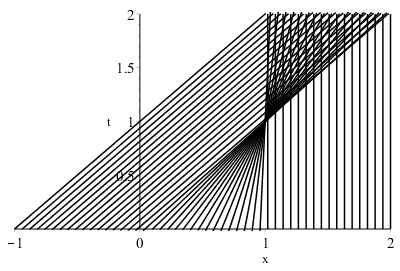
\includegraphics[width=0.5\linewidth]{./lect2/p2.png}
\end{center}

In point $x,y$ we have slope $u(x,y)$ thus the charecteristic curve crosses $x$-axis at $x_0 = x-uy$ and from initial conditions, $u=1-\frac{x_0}{\alpha}$. Thus
$$u=1-\frac{x-uy}{\alpha}$$
$$\alpha u=\alpha-x+uy$$
$$(\alpha-y) u=\alpha-x$$
Acquiring
$$u = \frac{x-\alpha}{y-\alpha}$$
And now for $y>1$ from Rankine–Hugoniot conditions
$$u(x,y) = \begin{cases}
1 & x<\alpha + \frac{1}{2} (y-\alpha)\\
0 & x>\alpha + \frac{1}{2} (y-\alpha)\\
\end{cases}$$
Such a solution is called a shock wave.

\begin{center}
	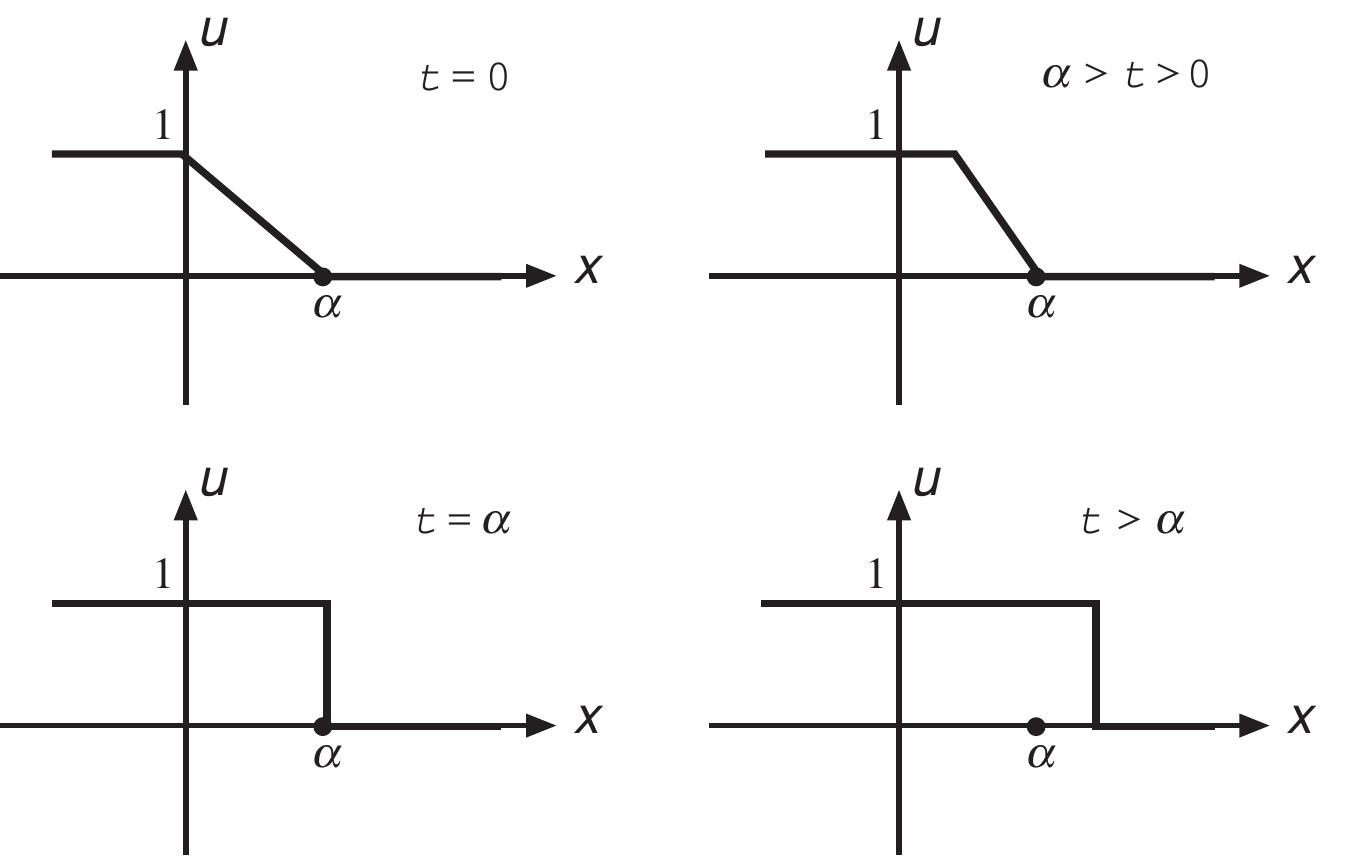
\includegraphics[width=0.7\linewidth]{./lect2/p1.png}
\end{center}

\paragraph{Example}
For
$$h(x) = \begin{cases}
0 & x> \alpha\\
1 & x < 0\\
\frac{x}{\alpha} & 0\leq x \leq \alpha
\end{cases}$$

Now there is no place where characteristic curves meet

\begin{center}
	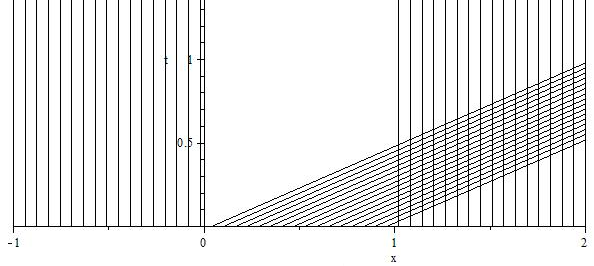
\includegraphics[width=0.7\linewidth]{./lect2/p3.png}
\end{center}

In the region without characteristic curves ($0\leq x\leq y$) we get the following: the solution starts from some  point $x_0 = x-uy$, and similarly to the previous case, from initial conditions,
$$u=\frac{x}{\alpha +y}$$


\begin{center}
	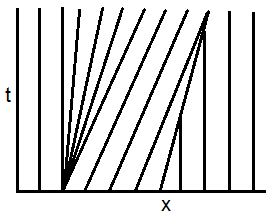
\includegraphics[width=0.3\linewidth]{./lect2/p4.png}
\end{center}

\paragraph{What happens if $\alpha \to 0$?}
We get $u=\frac{x}{y}$ for $0\leq x \leq y$. We acquired rarefaction wave - starting from something non-continuous we got continuous solution. This is weak solution.

However, also shock wave along $y=x$ is also solution of initial conditions. This solution is worse, because shock wave loses information, which means we cant reproduce the solution for some $y<y_0$ even if I know the values for $y=y_0$.
\paragraph{Entory principle}
Weak solution is unique if characteristic curves meet shock wave from direction of increasing time. 


\subsection{Fully non-linear equations}
\paragraph{Hamilton-Jacoby equation}
$$u_x^2+u_y^2=1$$
Can we generalize the method of solution of quasilinear equations to fully non-linear equations? The answer is yes. 
We have some $$F(x,y,u,u_x,u_y) = 0$$. In our case $$F(x,y,u,p,q) = p^2+q^2-1$$

Characteristic equations:
$$\begin{cases}
\dv{x}{t} = \pdv{F}{p}\\
\dv{y}{t} = \pdv{F}{q}\\
\dv{z}{t} = p\pdv{F}{p}+q\pdv{F}{q}\\
\dv{p}{t} = -\pdv{F}{x}+p\pdv{F}{z}\\
\dv{q}{t} = -\pdv{F}{y}+q\pdv{F}{z}\\
\end{cases}$$


Suppose we have initial curve $\Gamma = (\bar{x}(s), \bar{y}(s), \bar{z}(s))$

We need to find $\bar{p}$ and $\bar{q}$. We have two additional conditions:
$$F(x,y,u,u_x,u_y) = 0$$
also
$$u(\bar{x}(s), \bar{y}(s)) = \bar{z}(s)$$
Differentiating by $s$
$$\pdv{u}{x}\dv{\bar{x}}{s}  + \pdv{u}{y}\dv{\bar{y}}{s} = \dv{\bar{z}}{s}$$
$$\bar{p}(s)\dv{\bar{x}}{s} + \bar{q}(s)\dv{\bar{y}}{s} = \dv{\bar{z}}{s}$$
Now we can find $p$ and $q$.

Back to our equation:
$$\begin{cases}
\dot{x} = 2p\\
\dot{y} = 2q\\
\dot{z} = 2(p^2+q^2)\\
\dot{p} = \dot{q} = 0
\end{cases}$$

In case we have initial curve with $u=0$, then characteristic curves are perpendicular to initial curve.  We get $u(x,y)$ equal to distance from initial curve, since absolute value of gradient of $u$ is $1$ due to equation.

If we have $u=\phi(s)$ on initial curve, we acquire
$$u(x,y) = \min (x-\bar{x}(s))^2 + (y-\bar{y}(s))^2 + \phi(s)$$

\paragraph{Higher dimension}
We can trivially extend quasilinear equations to more dimensions. In this case we have initial surface instead of curve.
\section{Wave equation}
$$u_{tt} -c^2u_{xx} = 0$$
More generally, any second order linear equation can be written as
$$a(x,y) u_{xx} + 2b(x,y) u_{xy} + c(x,y) u_{yy} + du_x + eu_y + fu = g$$

\paragraph{Definition}
Equation is called hyperbolic if $b^2-ac>0$, parabolic if  $b^2-ac=0$ and elliptic if  $b^2-ac<0$. Wave equation is hyperbolic in the whole space.

We want to simplify the equation: we are searching for $\xi(x,y)$ and $\eta(x,y)$ such that
$$\pdv{\eta}{x} \pdv{\xi}{y} - \pdv{\eta}{y} \pdv{\xi}{x} \neq 0$$
and solution $u(x,y) = w\big(\xi(x,y), \eta(x,y)\big)$.

Derivatives of $u$ are
$$u_y = w_\xi \xi_y + w_\eta \eta_y$$
$$u_{yy} = w_{\xi\xi} \xi_{y}^2 + w_{\xi\eta}\xi_y\eta_y + w_{\xi}\xi_{yy} + w_{\eta \xi}\eta_y\xi_y + w_{\eta\eta} \eta_{y}^2+ w_{\eta}\eta_{yy}  $$
$$u_{xy} =\pdv{x}\pdv{u}{y} = w_{\xi \xi} \xi_x\xi_y + w_{\xi\eta}\xi_y\eta_x + w_{\xi\eta}\xi_x\eta_y + w_{\eta \xi} \eta_x\eta_y + w_{\xi}\xi_{xy}+w_\eta\eta_{xy}$$

Now we can get equation of form
$$A(\xi,\eta) w_{\xi\xi} + 2B(\xi,\eta) w_{\xi\eta} + C(\xi,\eta) w_{\eta \xi} + D(\xi,\eta) w_{\eta\eta}+ F(\xi,\eta) = 0$$
If we can find variable substitution such that
$$A=C=0$$
Then, in case of $d=e=f=0$,
$$Bw_{\xi\eta} = 0$$
i.e.,
$$w(\xi,\eta) = f(\xi)+g(\eta)$$